\section{Les différentes approches utilisées}
\begin{frame}{Modèle s'appuyant sur des règles}
	\begin{itemize}
		\item Utilisation d'algorithmes simples s'appuyant sur des règles prédéfinies (correspondance des préfixes et/ou motifs)
		\item Gérer grâce à des dictionnaires statiques ou des listes.
		\item Avantages~: Simplicité et rapidité de mise en œuvre
		\item Inconvénients~: Rigidité, difficulté à gérer des cas complexes
	\end{itemize}
	\begin{center}
		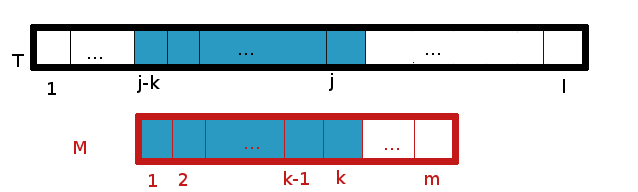
\includegraphics[width=\textwidth]{images/regles.png}
	\end{center}
\end{frame}

\begin{frame}{Modèle s'appuyant sur des statistiques}
	\begin{itemize}
		\item Utilisation de statistiques fournies grâce aux données d'un historique
		\item Prédire des séquence (Markov, TF-IDF)
		\item Avantages~: Résultats rapides et meilleure gestion des cas complexes.
		\item Inconvénients~: Pas de compréhension sémantique et besoin d'un grand nombre de données.
	\end{itemize}
	\begin{center}
		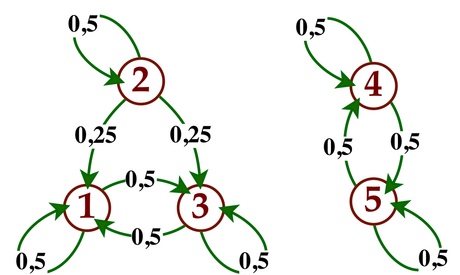
\includegraphics[width=0.5\textwidth]{images/statistiques.png}
	\end{center}
\end{frame}


\begin{frame}{Modèle s'appuyant sur l'intelligence artificielle}
	\begin{columns}
		\column{0.6\textwidth}
		\begin{itemize}
			\item Utilisation d'algorithmes s'appuyant sur l'intelligence artificielle et les réseaux neuronaux
			\item Apprentissage de motifs complexes à partir de données (forêt aléatoires, régressions pour plus de contexte)
			\item Avantages~: Efficace face à des cas complexes et des demandes rares, adaptabilité
			\item Inconvénients~: Nécessite beaucoup de temps de calcul et de ressources
		\end{itemize}
		\column{0.4\textwidth}
		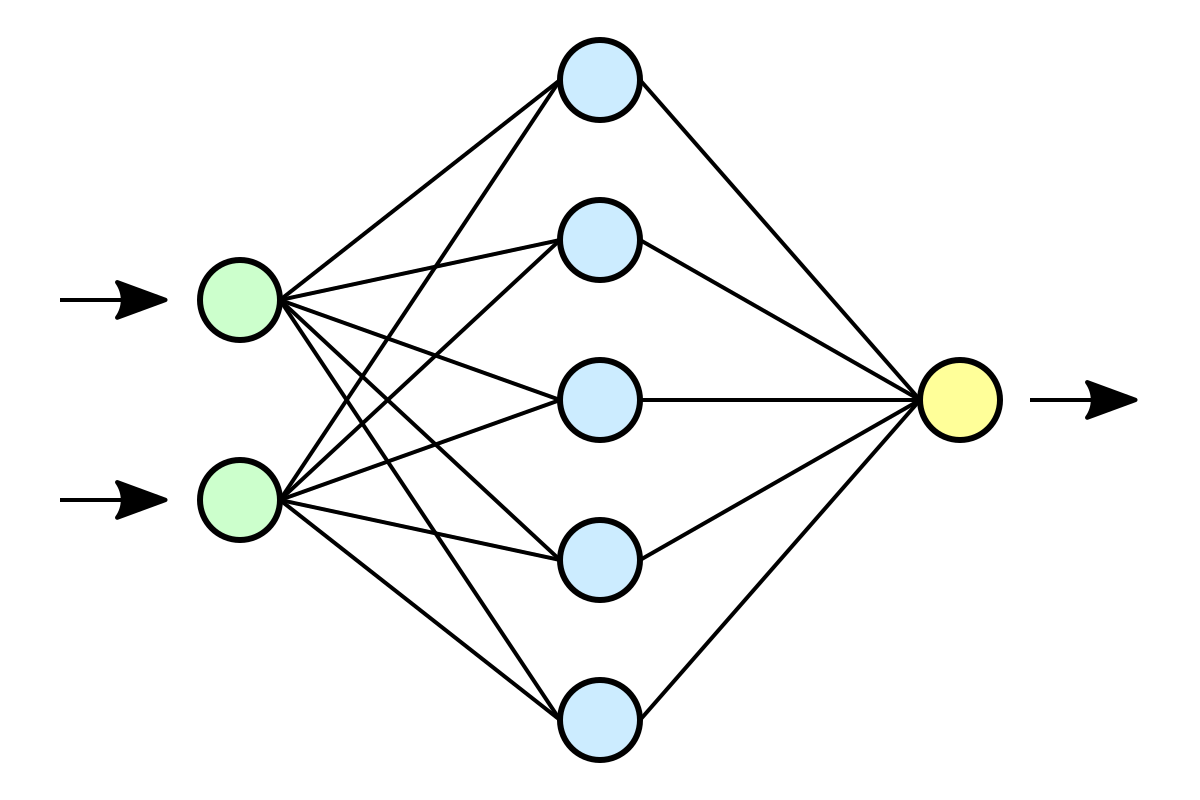
\includegraphics[width=\textwidth]{images/intelligence.png}
	\end{columns}
\end{frame}


\begin{frame}{Modèle s'appuyant sur l'amélioration continue}
	\begin{itemize}
		\item Utilisation d'algorithmes s'appuyant sur l'amélioration en temps réel.
		\item Choix fait par l'utilisateur, choix mémorisés pour une utilisation personnalisée
		\item Avantages~: Implémentation adaptable et avec des suggestions qui ont un sens sémantique, performance très élevée.
		\item Inconvénients~: Implémentation très complexes et longue à déployer, dépend des données collectées et des utilisateurs.
	\end{itemize}
	\begin{center}
		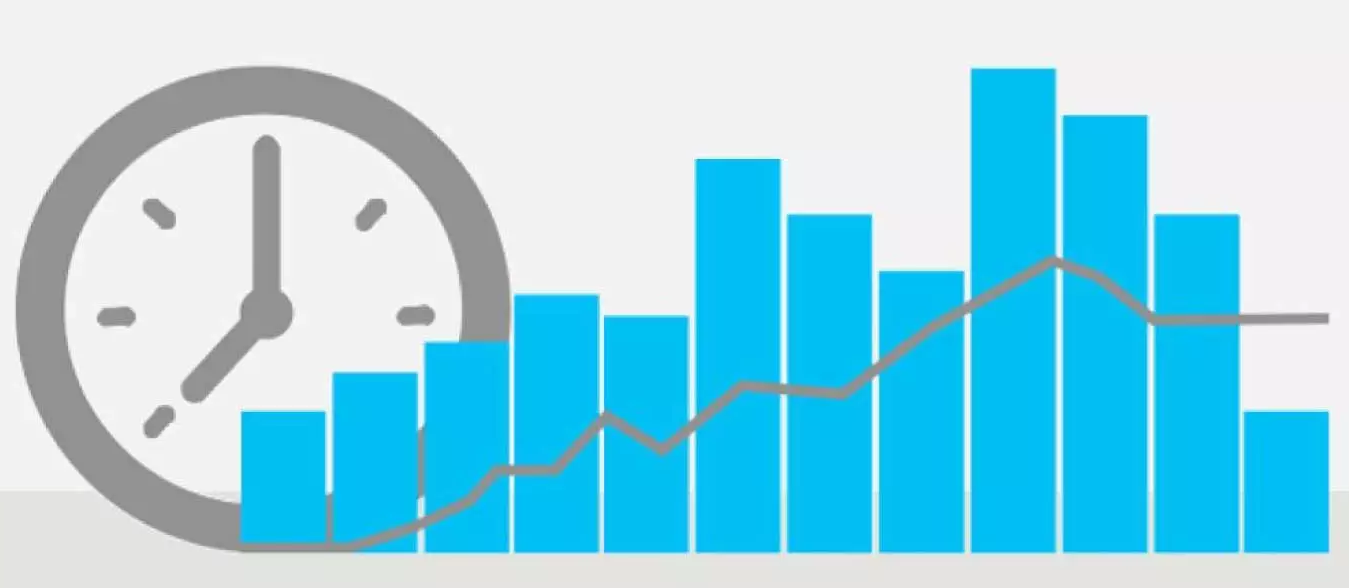
\includegraphics[width=0.6\textwidth]{images/learning.png}
	\end{center}
\end{frame}
